\documentclass{article}

% Language setting
% Replace `english' with e.g. `spanish' to change the document language
\usepackage[english, russian]{babel}

% Set page size and margins
% Replace `letterpaper' with `a4paper' for UK/EU standard size
\usepackage[letterpaper,top=2cm,bottom=2cm,left=3cm,right=3cm,marginparwidth=1.75cm]{geometry}

% Useful packages
\usepackage{amsmath}
\usepackage{graphicx}
\graphicspath{ {./images/} }
\usepackage[colorlinks=true, allcolors=blue]{hyperref}
\usepackage[T2A]{fontenc}


\title{Сравнение стратегий в многоруких бандитах для распределения Стьюдента с разными степенями свободы}
\author{Михаил Давыдов}

\begin{document}
\maketitle

\section{Методология}

Для рассмотрения алгоритмов я использовал 10 рычагов, распределения всех рычагов одинаковы с точностью до смещения. Я рассмотрел 4 распределения: стандартное нормальное распределение ($\mathcal{N}(0,1)$ или $t_{\infty}$), которое является предельным случаем распределения Стьюдента при числе степеней свободы, стремящемся к бесконечности; распределение Стьюдента с 3 степенями свободы ($t_3$), домноженное на $\frac{1}{\sqrt{3}}$, чтобы дисперсия была равна 1; распределение Стьюдента с 2 степенями свободы ($t_2$) без нормировки, поскольку у $t_2$ нет дисперсии; распределение Стьюдента с 1 степенью свободы, или же стандартное распределение Коши ($t_1$). Каждое из этих распределений было смещено на значение, выбранное случайно из $\mathcal{N}(0,1)$.

Стратегии и порядок проверки распределений полностью совпадают с таковыми в описанной выше книге Саттона и Барто, а именно:
\begin{enumerate}
    \item Рассматриваются $\epsilon$-greedy стратегии, то есть стратегии, действия в которых выбираются по формуле
    $$A_t = \begin{cases}
            \underset{a}{\arg \max} \; Q_t(a), & \text{with probability} \; 1 - \epsilon, \\
            \text{a random action}, & \text{with probability} \; \epsilon.
            \end{cases}$$ 
    (среди равных значений выбор происходит случайно). Далее выбираются $\epsilon$-greedy стратегии с $\epsilon = 0$ (то есть просто жадная стратегия), $0.01, 0.1$. Изначально $\forall a \; Q_t(a) = 0$.
    \item Далее берутся стратегии с оптимистичной инициализацией, то есть стратегии, для которых изначально $\forall a \; Q_t(a) = d, \; d > 0$. Я использовал $d=5$ (как в книге). Обновление $Q_t(a)$ происходит с константынм шагом, то есть если на шаге $t$ было выбрано действие $a$, то для всех остальных действий $b$ значение $Q_t(b)$ не меняется, а для действия $a$ $Q_t(a) = Q_t(a) + \alpha (R_t - Q_t(a)), \; \alpha = const$. $\alpha$ называется step-size. Так же, как и в книге, я выбрал $\alpha = 0.1$. Я сравнил greedy-стратегию с оптимистичной инициализацией с $0.1$-greedy стратегиями с обычной и оптимистичной инициализациями.
    \item Upper-Confidence-Bound Action Selection -- выбор действия происходит по формуле 
    $$A_t = \underset{a}{\arg \max} \; \left[ Q_t(a) + c \sqrt{\frac{ln \; t}{N_t(a)}} \right], \; c > 0$$
    В случае, когда $N_t(a) = 0$, значение функции справа считается равным бесконечности. Сравнил UCB с $c = 2$ с $0.1$-greedy стратегией.
    \item Gradient bandits: для каждого действия $a$ вводится значение $H_t(a)$. На $t$-ом шаге выбор происходит среди действий соответственно вероятностям $\Pr\{A_t = a\} = \frac{e^{H_t(a)}}{\sum_{i=1}^{k} e^{H_t(i)}} := \pi_t(a)$. После выбора действия $A_t$ и получения награды $R_t$ обновления $H_t$ происходят по формулам:
    $$\begin{aligned}
      H_{t+1}(A_t) = H_t(A_t) + \alpha (R_t - \bar{R_t}) (1 - \pi_t(A_t)), \; \text{and} \\ 
      H_{t+1}(a) = H_t(a) - \alpha (R_t - \bar{R_t})\pi_t(a), \; a \neq A_t.
      \end{aligned}$$
    Я сравнил результаты gradient bandits для $\alpha = 0.1, \; 0.4$, и в случаях, когда baseline есть и когда его нет. При этом моды распределений специально смещены на 4, чтобы показать, что, в отличие от других стратегий gradient bandit невосприимчив к смещению распределений.
\end{enumerate}

Каждую из стратегий я запустил для каждого из распределений на 2000 независимых тестах (для каждого теста свое смещение распределений) длиной 1000 шагов каждый, после чего посчитал среднюю награду и процент выбранных оптимальных действий на каждом шагу (во всех распределениях оптимальным считался рычаг с наибольшей медианой, что в случае нормального и Стьюдента с 
 $> 1$ степеней свободы равносильно наибольшему матожиданию). Для каждого распределения и каждой метрики результаты для одной группы стратегий визуализированы на графике. Кроме того, я решил дополнительно изобразить для каждой стратегии и для каждой метрики на одном графике результаты по всем распределениям.

 В конце я провел обзор всех стратегий для различных значений гиперпараметров. Для каждой стратегии варьировался один ключевой гиперпараметр, варьирование происходило по значениям $$ \frac{1}{128}, \frac{1}{64}, \frac{1}{32}, \frac{1}{16}, \frac{1}{8}, \frac{1}{4}, \frac{1}{2}, 1, 2, 4$$ (для $\epsilon$-greedy значения 2 и 4 не рассматривались). Взяты стратегии:
 \begin{itemize}
     \item $\epsilon$-greedy, варьирование по $\epsilon$
     \item greedy с оптимистичной инициализацией и $\alpha = 0.1$, варьирование по $Q_0(a)$
     \item UCB, варьирование по $c$
     \item gradient bandits, варьирование по $\alpha$
 \end{itemize}
 
 Ввиду долгого выполнения процент оптимальных действий и средняя награда брались по 1000 тестам, при этом количество шагов осталось равным 1000. В случае средней награды бралась средняя награда на 1000-ом шагу, в случае оптимального действий брался наилучший процент за 1000 шагов. Все эти вычисления были выполнены для всех распределений, после чего для каждого распределения и для каждой метрики значения были визуализированы на графике.

 Сам код можно найти \href{https://github.com/davynchi/diploma/blob/main}{в этом репозитории} в папке "gradient bandit".

\section{Результаты}

На всех графиках график средней награды для распределения Коши не имеет смысла ввиду отсутствия у распределения матожидания.

\begin{enumerate}
    \item $\epsilon$-greedy: Как можно видеть, для $t_2, t_3, t_{\infty}$ при увеличении $\epsilon$ до значения $\frac{1}{k} = \frac{1}{10}$ средняя награда и процент оптимальных действий увеличиваются. Для $t_2$ характерны резкие прыжки в средней награде ввиду отсутствия дисперсии. Для $t_1$ процент оптимальных действий значительно ниже других распределений и составляет около $30\%$, более того, оптимальный процент действий для каждой из стратегий примерно одинаков, изменение $\epsilon$ не ведет к изменению процента оптимальных действий для $t_1$. Предположу, что при $\nu \to 0$ процент оптимальных действий $t_{\nu}$ стремится к $\frac{1}{k}$. При положительном $\epsilon$ средняя награда и процент оптимальных действий для $t_3$ и $t_{\infty}$ примерно одинаковы, а для $t_2$ эти значения несколько ниже. Для greedy стратегии наблюдается другая картина: метрики для $t_{\infty}$ выше, чем для $t_3$, что можно объяснить тем, что после сжатия $t_3$ его пик стал более острым, и более резких изменений стало меньше, чем у $t_{\infty}$, из-за чего исправлений неправильных выборов рычагов стало меньше. Для $t_2$ наоборот, метрики выше, чем у $t_{\infty}$, что объясняется отсутствием дисперсии и более частыми ``далекими'' значениями, что повышает вероятность исправления неправильных выборов рычагов.
    \begin{figure}
        \centering
        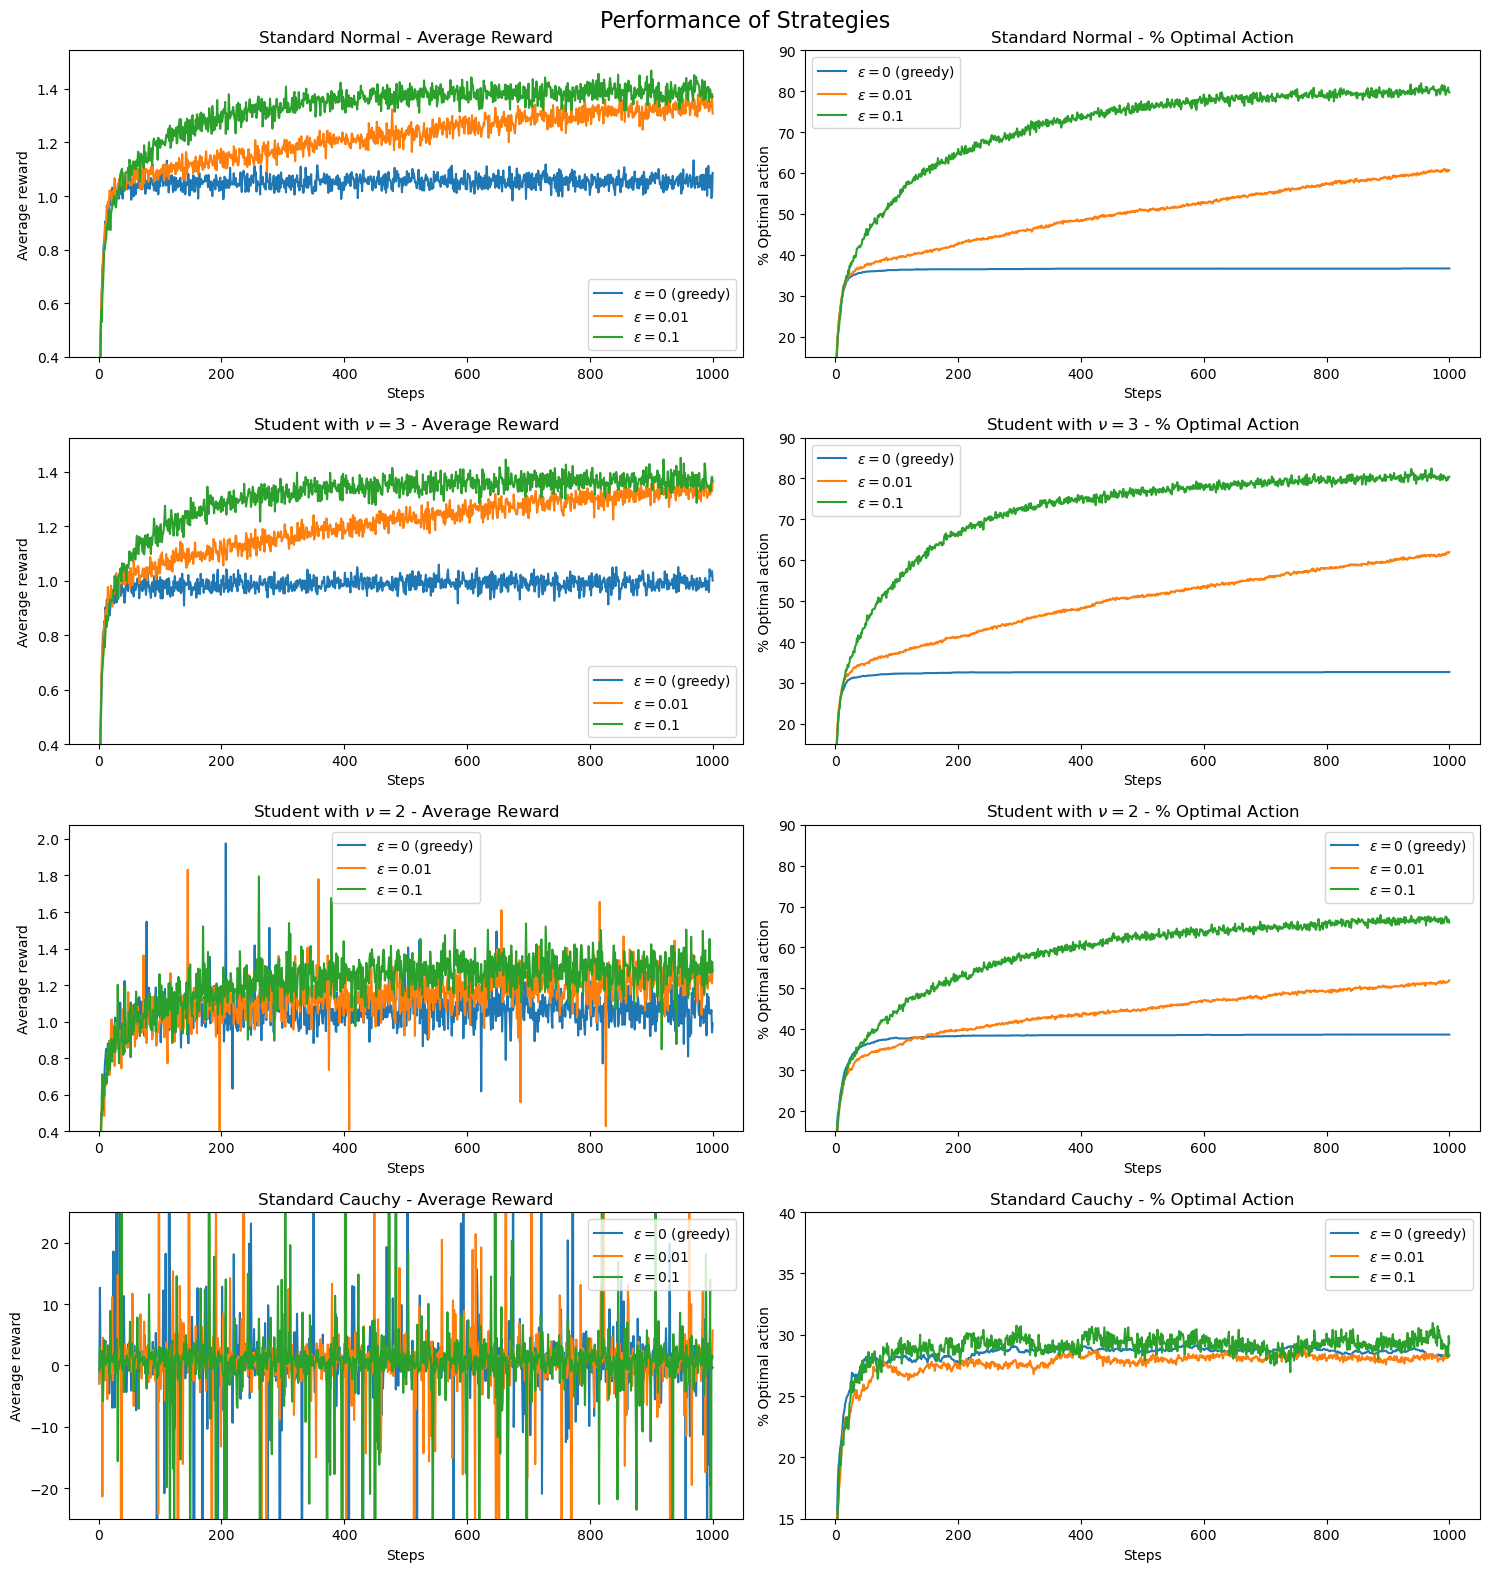
\includegraphics[width=1.1\linewidth]{eps_greedy_1.jpg}
        \caption{\label{fig:eps_greedy_1}Значения средней награды и процента оптимального выбора для $\epsilon$-greedy стратегий, сгруппировано по распределениям}
    \end{figure}
    \begin{figure}[t]
        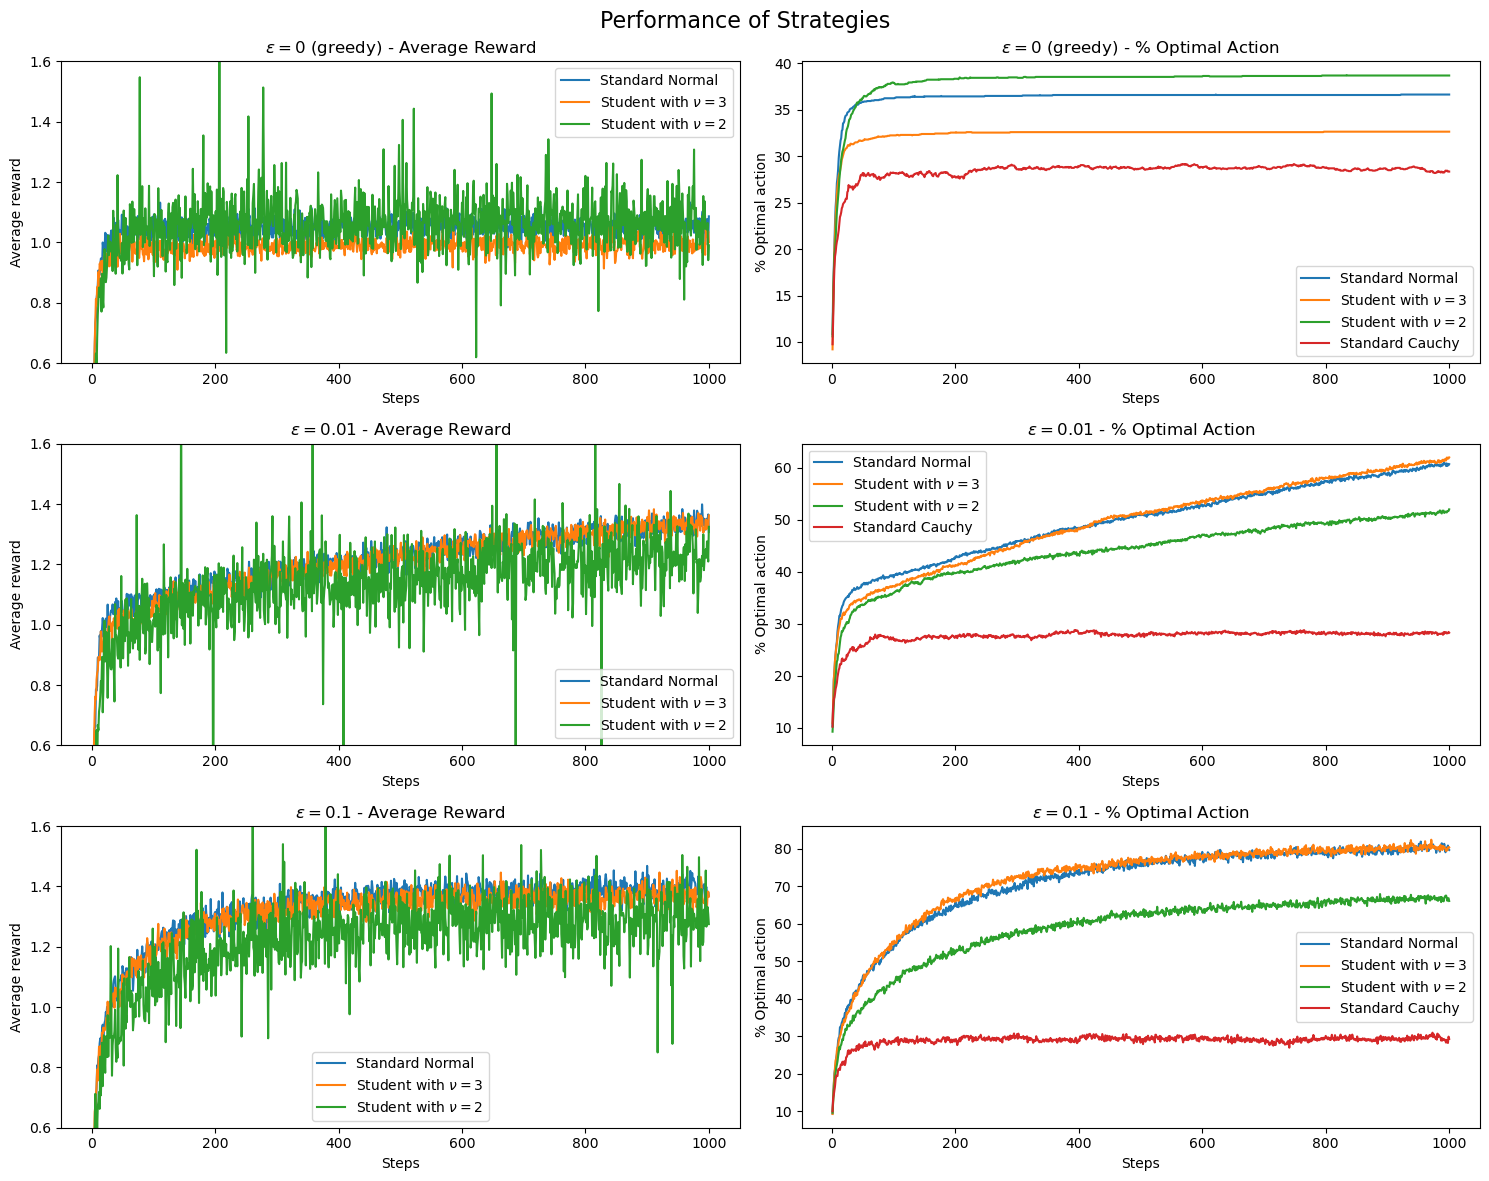
\includegraphics[width=1.1\linewidth]{eps_greedy_2.jpg}
        \caption{\label{fig:eps_greedy_1}Значения средней награды и процента оптимального выбора для $\epsilon$-greedy стратегий, сгруппировано по стратегиям}
    \end{figure}
    \item Оптимистичная инициализация: здесь ситуация несколько отличается. Оптимистичная жадная стратегия лучше оптимистичной $\epsilon$-greedy и реалистичной $\epsilon$-greedy только для $t_{\infty}$ и $t_3$, причем для $t_3$ процент оптимальных действий для всех трех стратегий выравнивается к 1000-му шагу. Для $t_2$ и $t_1$ средняя награда и процент оптимальных действий для оптимистичной жадной стратегии хуже, чем для остальных стратегий. То есть жадность стратегии сильнее влияет на результат, чем инициализация. При этом для всех распределений для $\epsilon$-greedy оптимистичной и реалистичной стратегий средняя награда и процент оптимальных действий выравниваются, что объясняется маленьким вкладом начальной инициализации на 1000-ом шагу. Кроме того, для $t_3, t_2, t_1$ и константного step-size наблюдается переобучение: в какой-то момент средняя награда и процент оптимальных действий начинают падать. Такая проблема возникает в силу того, что для константного step-size вклад выбросов не уменьшается со временем, и потому для распределений с тяжелыми хвостами возникает ситуация, когда приход ``выброса'' резко изменяет среднюю награду оптимального действия в отрицательную сторону, и затем это действие выбирается гораздо реже. Аналогично предыдущему эксперименту, для $t_2$ виден разброс в средней награде из-за отсутствия дисперсии.
    Если сравнивать распределения, то с уменьшением степеней свободы обе метрики падают. При этом для $t_2$ высота пика в проценте оптимальных действий на 10-ом шагу выше, чем для $t_{\infty}$, что опять же, можно объяснить большей остротой пика.
    \begin{figure}
        \centering
        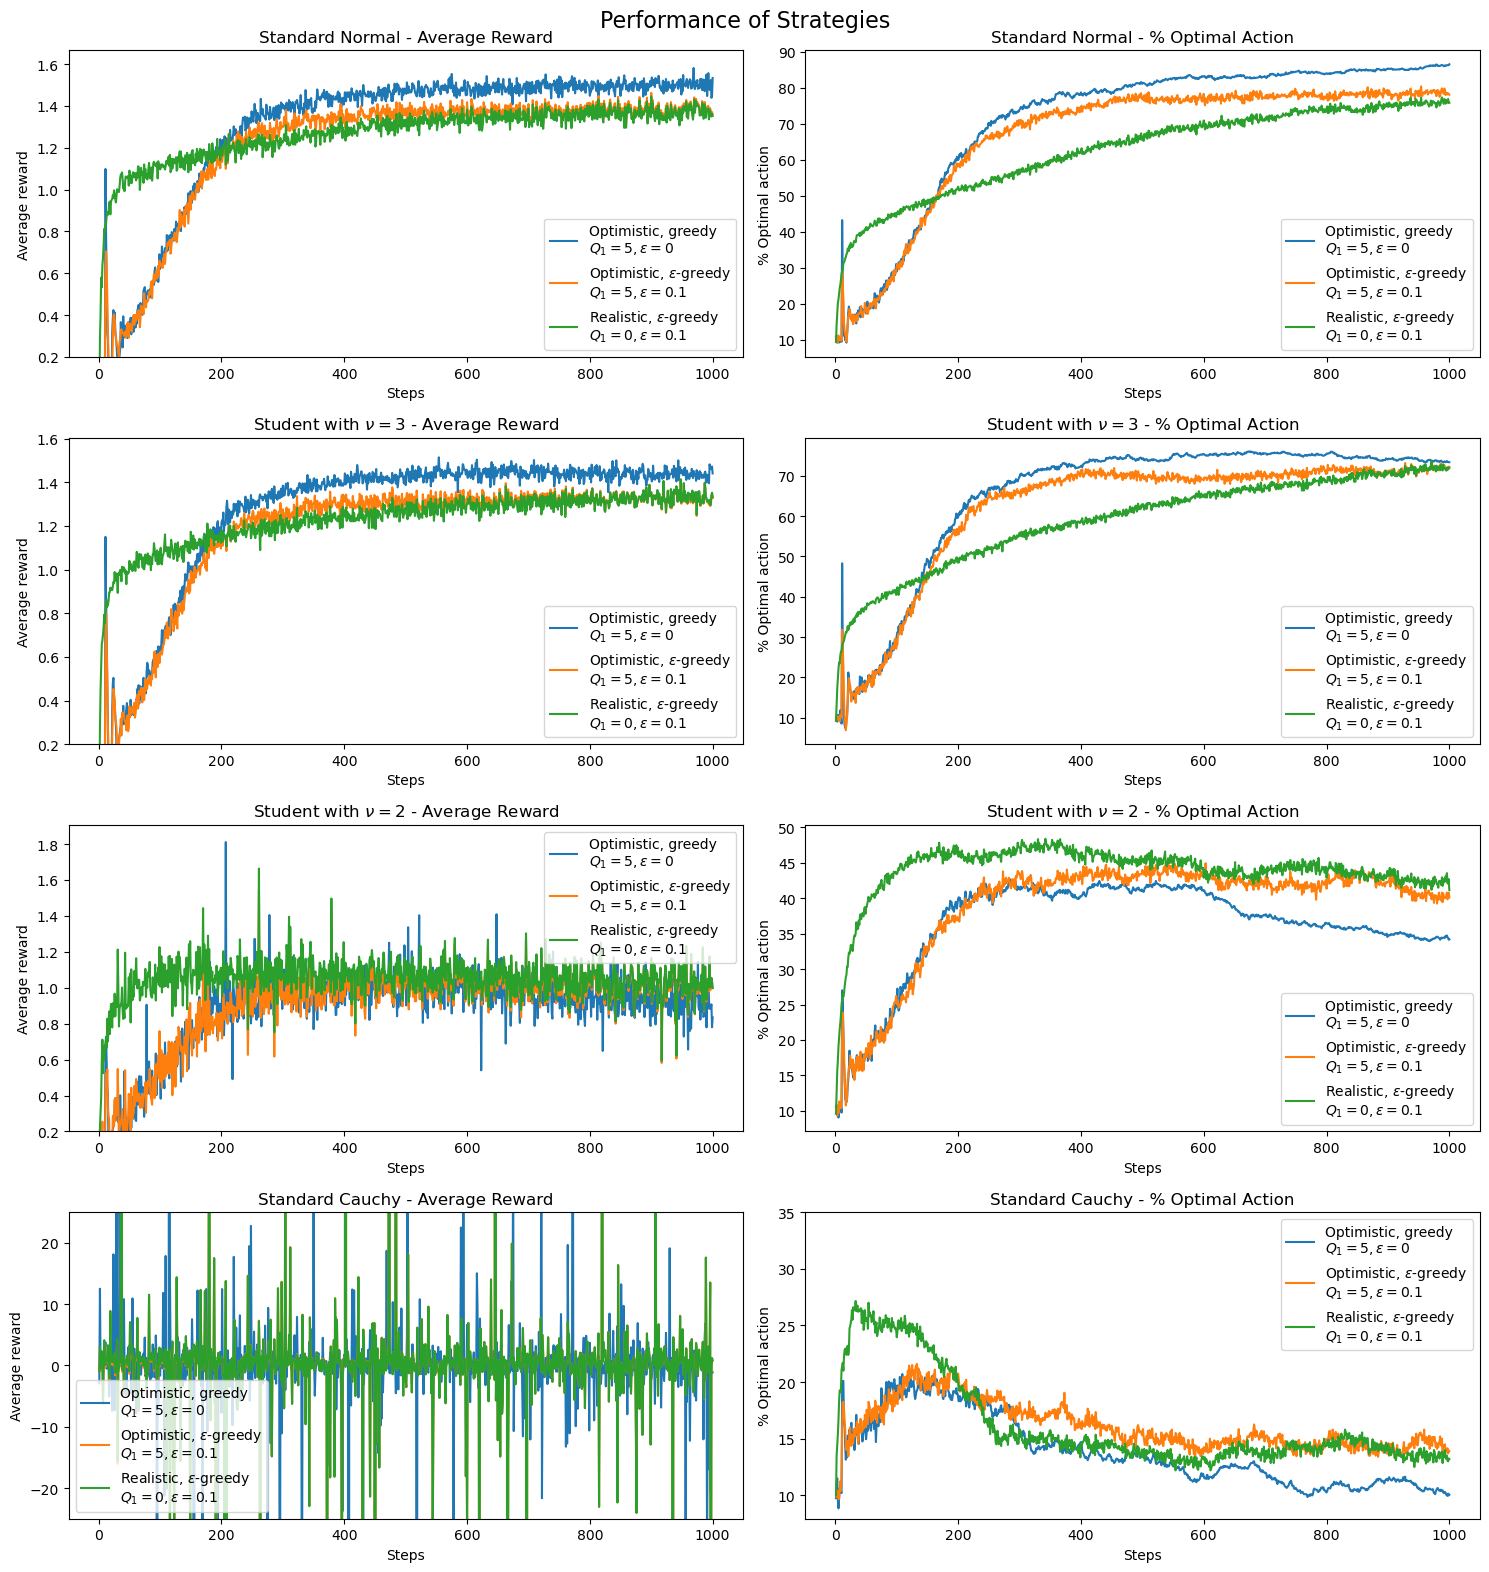
\includegraphics[width=1.1\linewidth]{optimistic_1.jpg}
        \caption{\label{fig:optimistic_1}Значения средней награды и процента оптимального выбора для оптимистичной стратегии в сравнении с $\epsilon$-greedy стратегий для константного step-size, сгруппировано по распределениям. Для $t_3, t_2, t_1$ видно переобучение}
    \end{figure}
    \begin{figure}[t]
        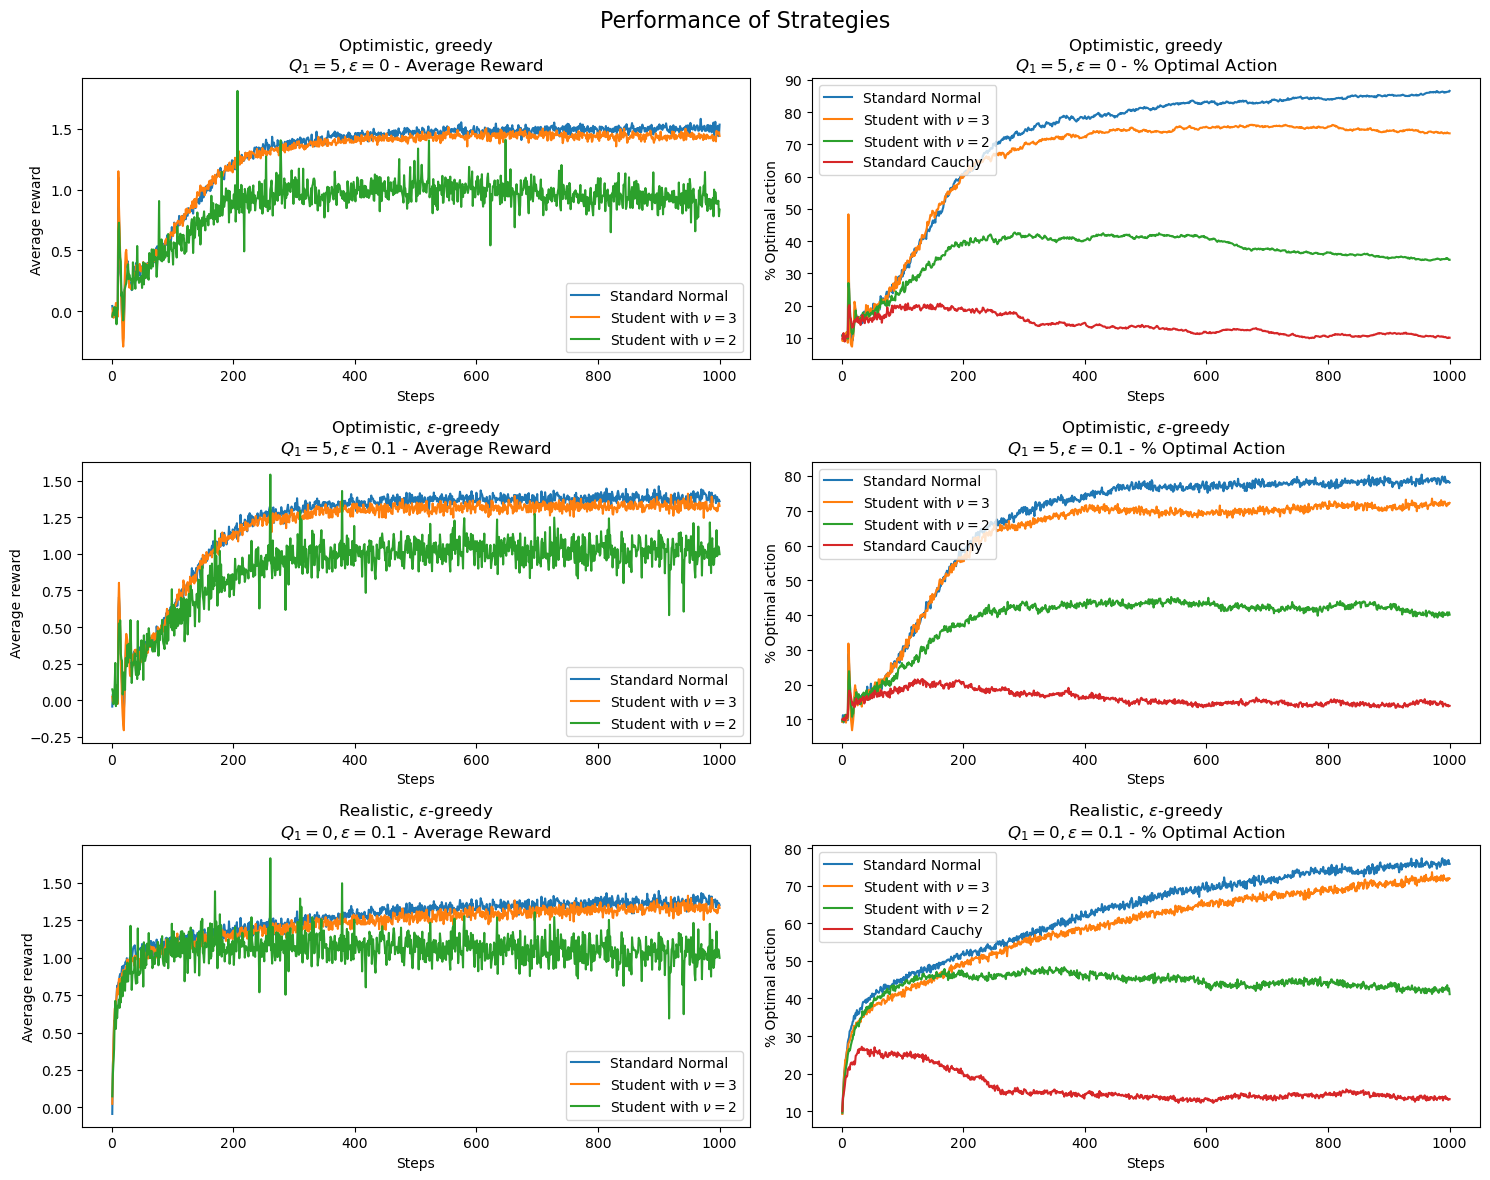
\includegraphics[width=1.1\linewidth]{optimistic_2.jpg}
        \caption{\label{fig:optimistic_2}Значения средней награды и процента оптимального выбора для оптимистичной и $\epsilon$-greedy стратегий для константного step-size, сгруппировано по стратегиям.}
    \end{figure}
    \item UCB: на всех распределениях и всех метриках видно, что UCB лучше $\epsilon$-greedy стратегии. Это можно объяснить тем, что UCB с увеличением уверенности реже производит "исследование" действий. При этом с уменьшением числа степеней свободы средняя награда незанчительно падает, а процент оптимальных действий падает заметно. Для $t_{\infty}$ и $t_3$ метрики падают на очень малую величину, позволяющую сказать, что UCB одинаково применимо для $t_{\infty}$ и $t_3$.
    \begin{figure}
        \centering
        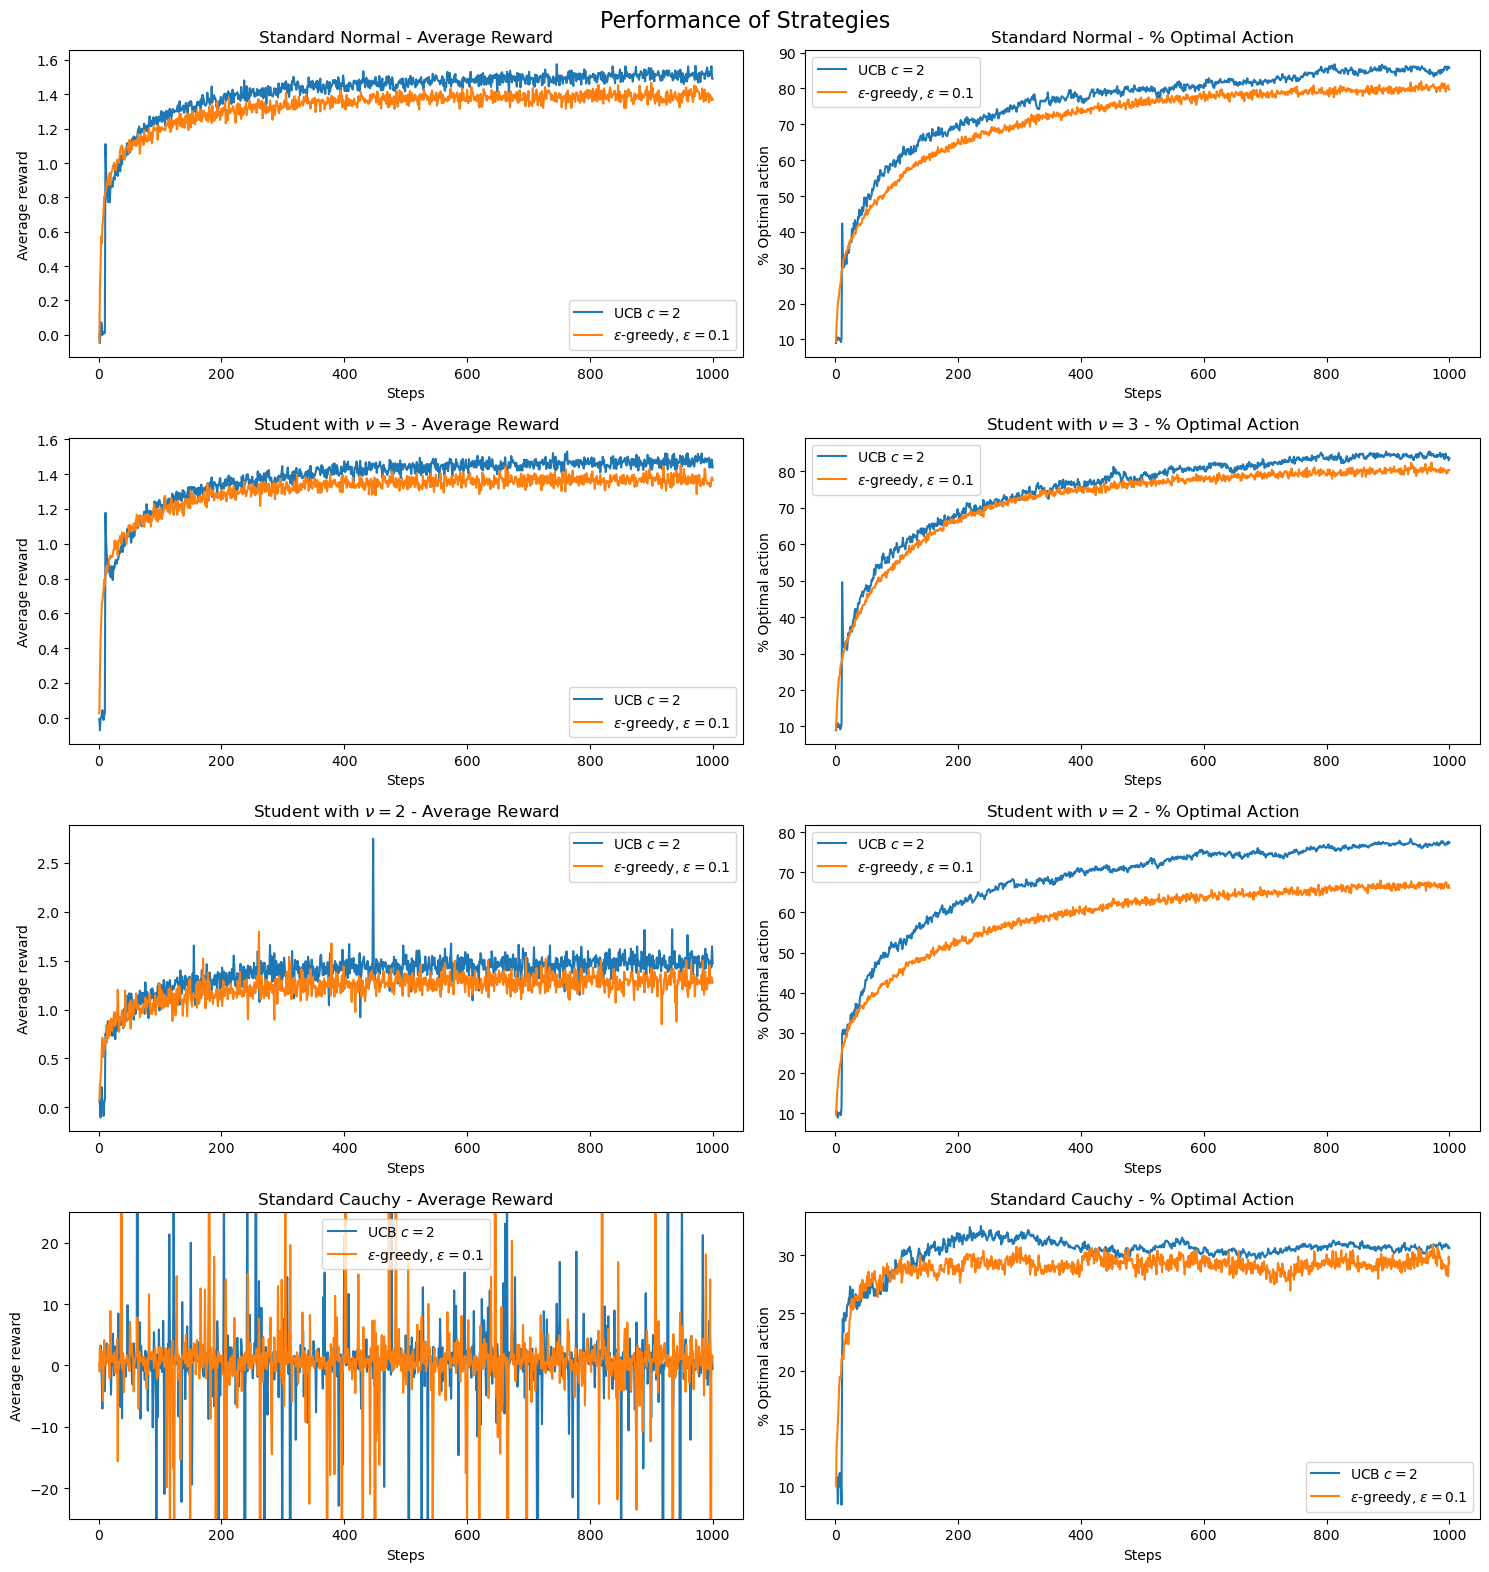
\includegraphics[width=1.1\linewidth]{ucb_1.png}
        \caption{\label{fig:ucb_1}Значения средней награды и процента оптимального выбора для UCB в сравнении с $\epsilon$-greedy, сгруппировано по распределениям. UCB лучше $\epsilon$-greedy на всех распределениях}
    \end{figure}
    \begin{figure}[t]
        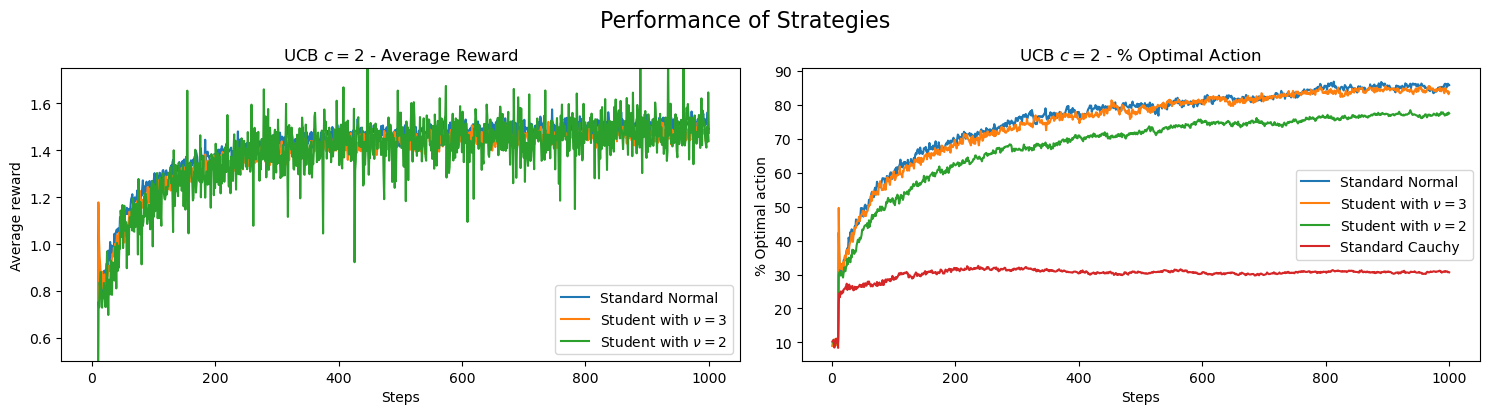
\includegraphics[width=1.1\linewidth]{ucb_2.png}
        \caption{\label{fig:ucb_2}Значения средней награды и процента оптимального выбора для UCB, сгруппировано по стратегиям.}
    \end{figure}
    \item Gradient bandits: для всех распределений присутствие baseline повышает значения метрик. Кроме того, значения метрик при $\alpha=0.1$ лучше, чем при $\alpha=0.4$ при заданных распределении и baseline, поскольку изменение $H_t(a)$ и, значит, $\pi_t(a)$, происходит менее резко, и выбросы меньше влияют на результат. С уменьшением $\nu$ разрыв в проценте оптимальных действий для для $\alpha=0.4$ с baseline и $\alpha=0.1$ без baseline сокращается, а для $t_1$ и вовсе почти совпадают, что дает говорить о том, что с уменьшением числа степеней свободы влияние baseline уменьшается. Впрочем, при $\nu < 1$ само понятие выборочного среднего как приближение матожидания перестает иметь смысл. Аналогично предыдущим пунктам, для $t_2$ и $t_1$ значение метрик ниже, чем для $t_3$ и $t_{\infty}$. Причем при увеличении $\alpha$ в ситуации с пристусттвием baseline значения метрик для $t_{\infty}$ становятся ниже, чем для $t_3$, при отсутствии baseline ситуация ровно наоборот.
    \begin{figure}
        \centering
        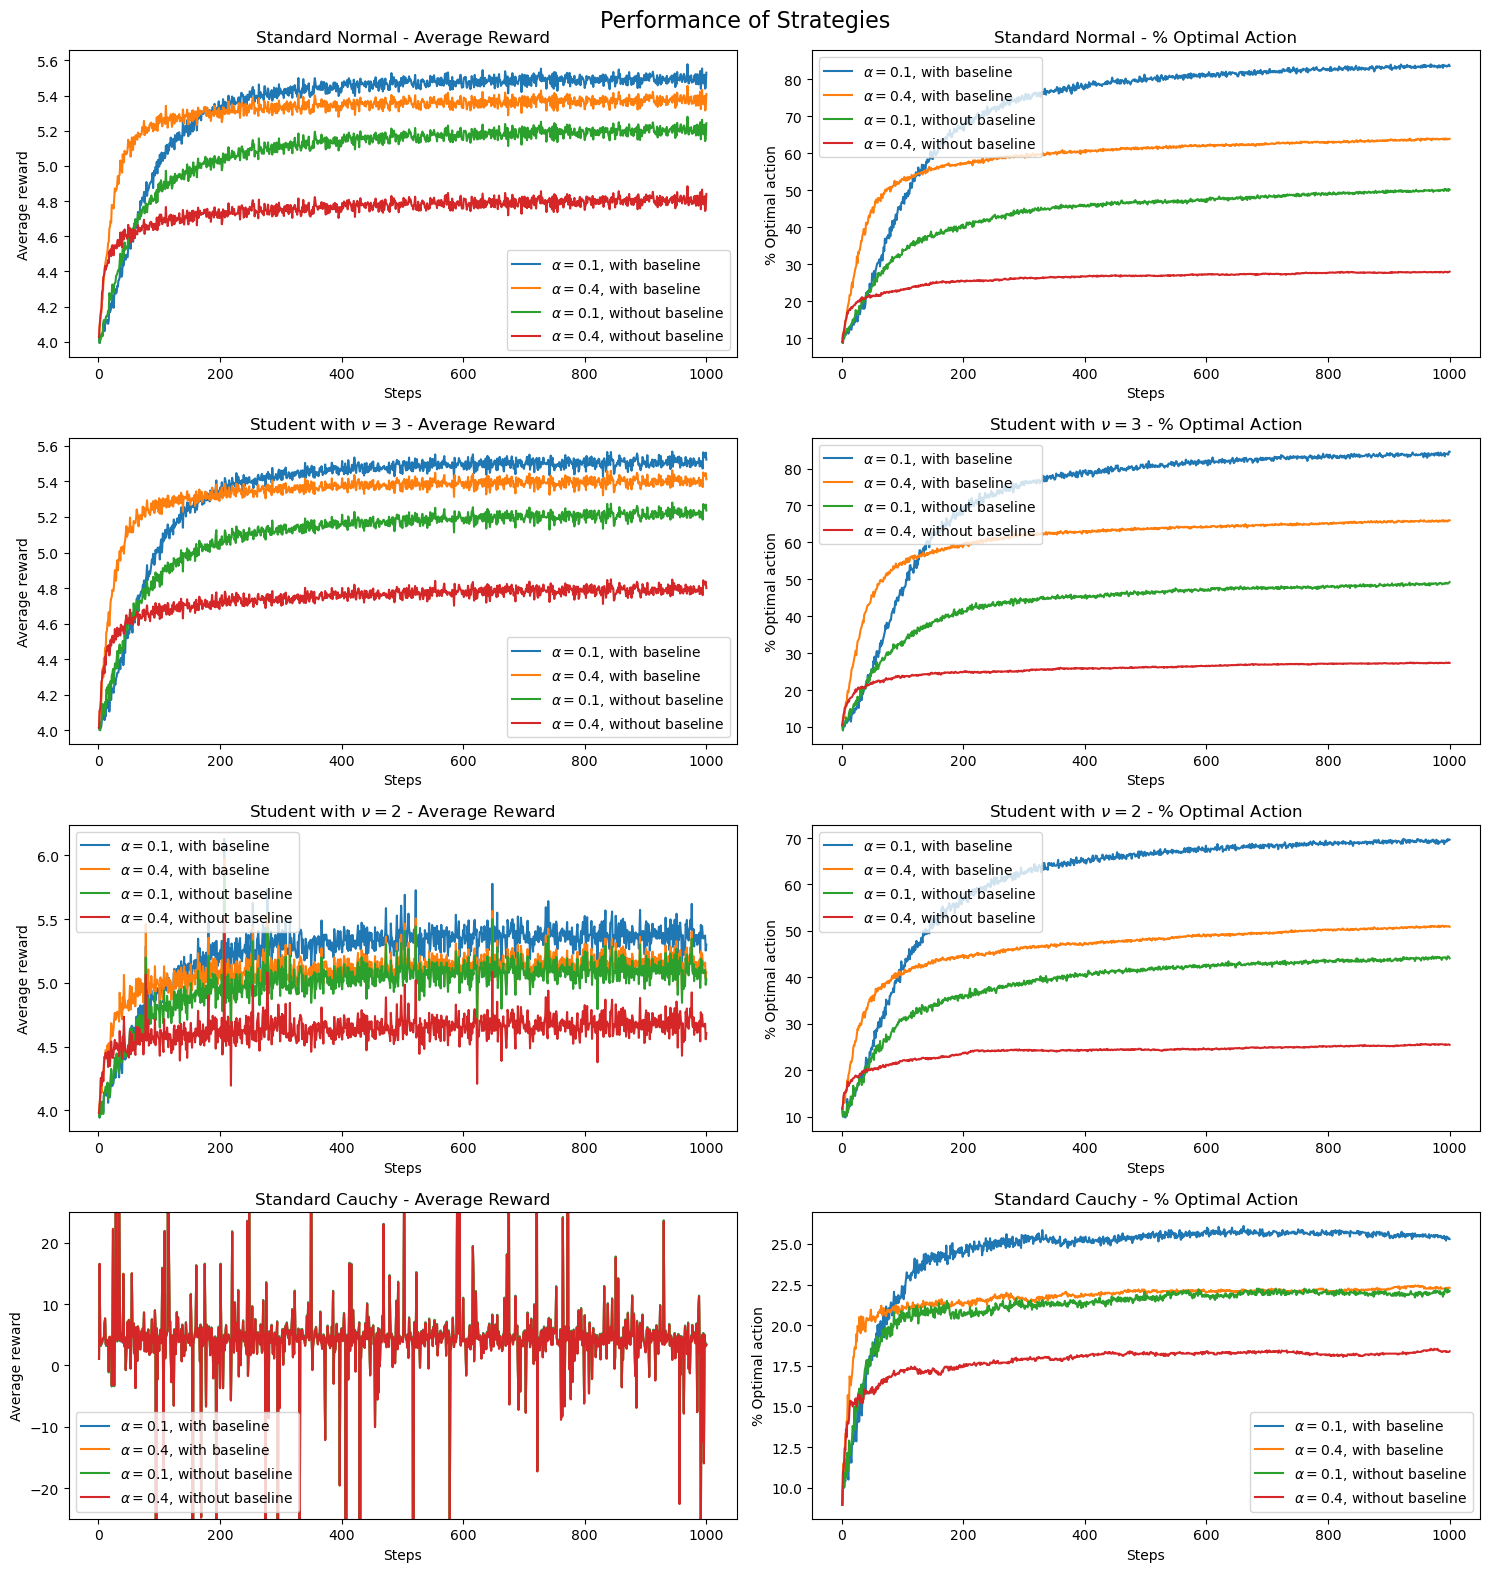
\includegraphics[width=1.1\linewidth]{gradient_1.png}
        \caption{\label{fig:gradient_1}Значения средней награды и процента оптимального выбора для gradient bandits, сгруппировано по распределениям. Меньшее $\alpha$ и присутствие baseline приводят к лучшим результатам}
    \end{figure}
    \begin{figure}[t]
        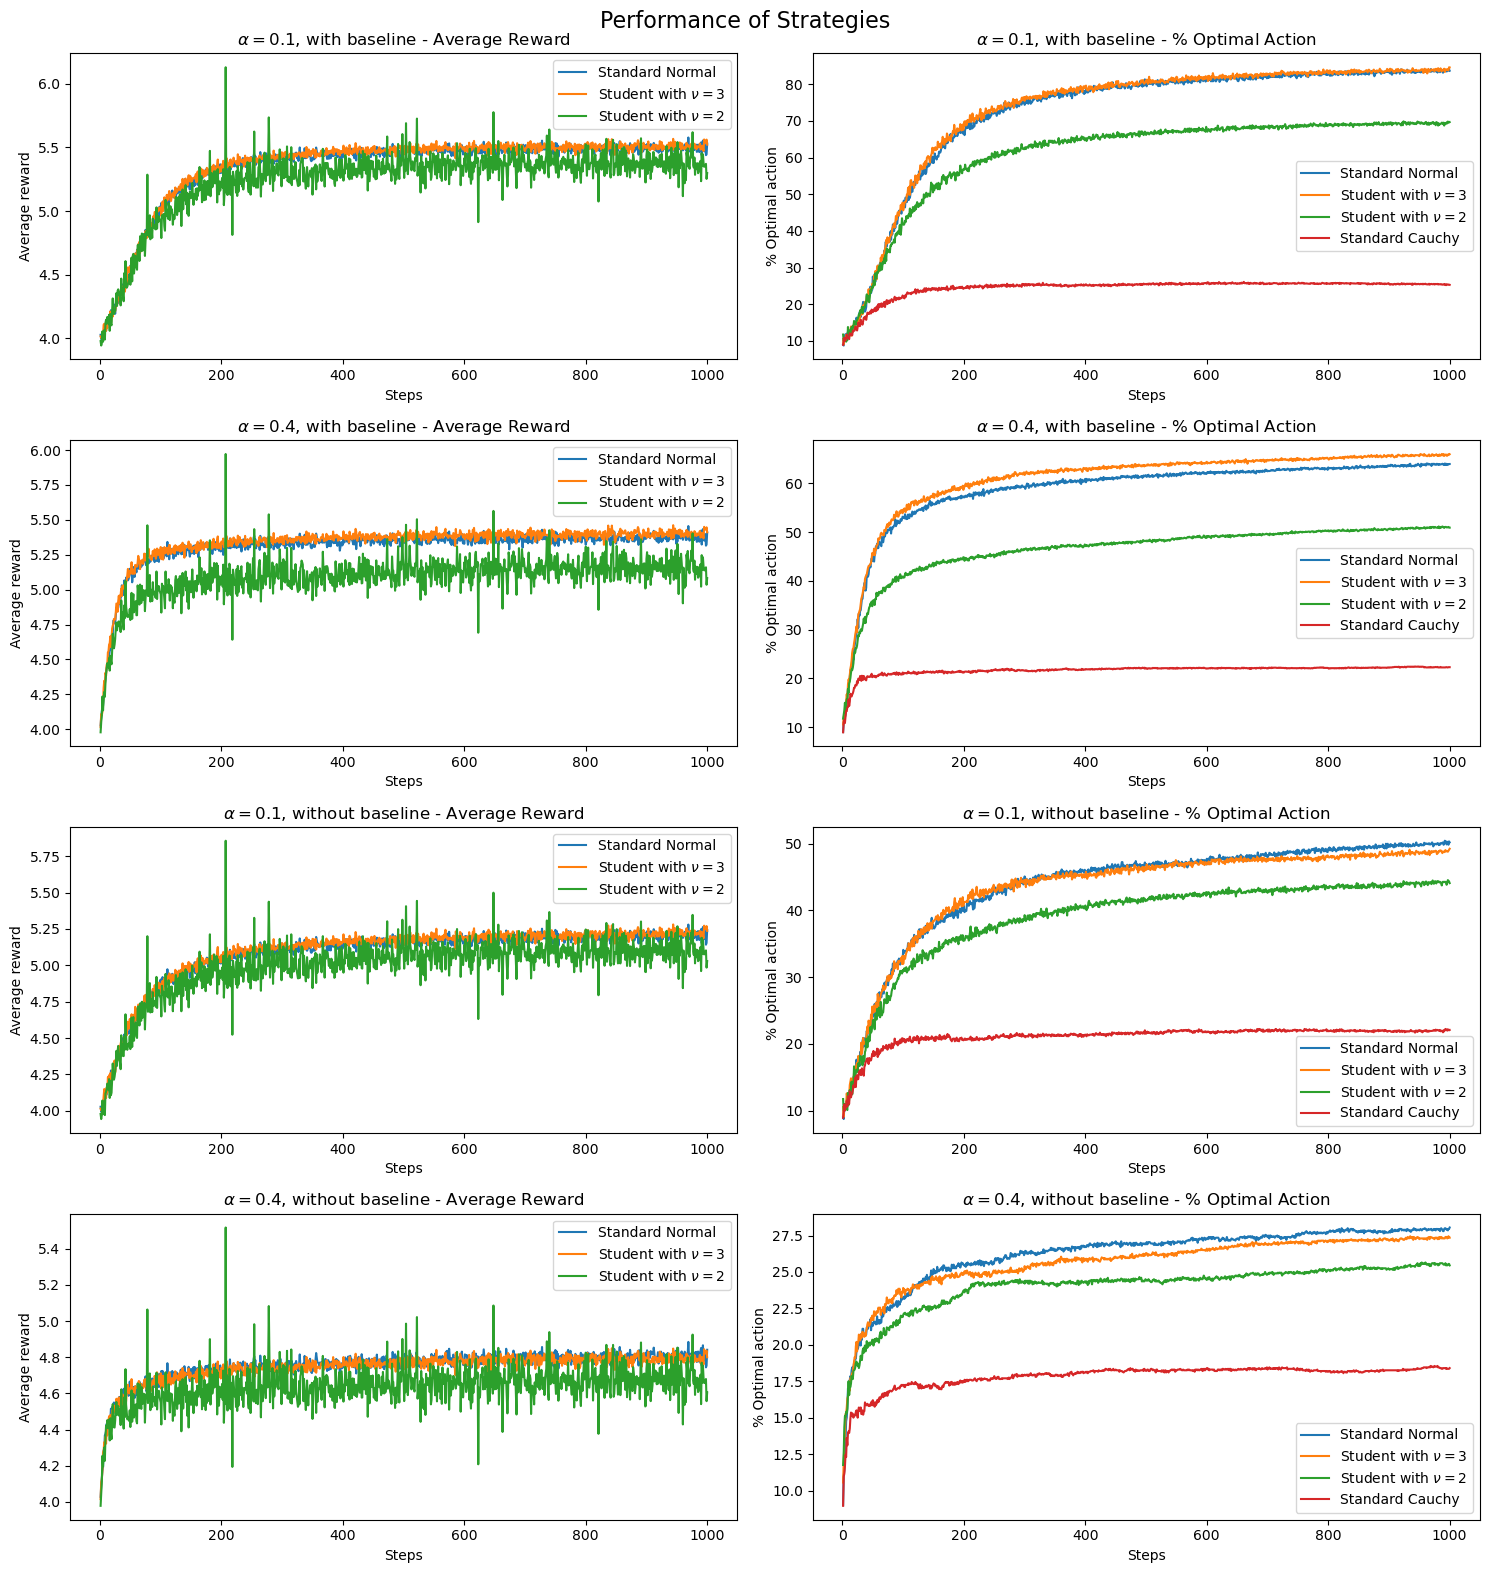
\includegraphics[width=1.1\linewidth]{gradient_2.png}
        \caption{\label{fig:gradient_2}Значения средней награды и процента оптимального выбора для gradient bandits, сгруппировано по стратегиям. Заметно странное поведение метрик: когда есть baseline, значения для $t_3$ лучше, чем для $t_{\infty}$}.
    \end{figure}
\end{enumerate}

В целом, характерны следующие тенденции:
\begin{enumerate}
    \item Везде, кроме greedy стратегий и стратегий с постоянным step-size, при увеличении числа степеней свободы значения метрик увеличиваются (или незначительно уменьшаются).
    \item У $t_2$ имеются резкие перепады в средней награде с сохранением тенденции к увеличению (или уменьшению для постоянного step-size). Это объясняется отсутсвием у $t_2$ дисперсии.
    \item Везде, кроме greedy стратегий и стратегий с постоянным step-size, занчения метрик для $t_{\infty}$ и $t_3$ почти совпадают, то есть стратегии одинаково применимы для этих двух распределений.
\end{enumerate}

\begin{figure}
    \centering
    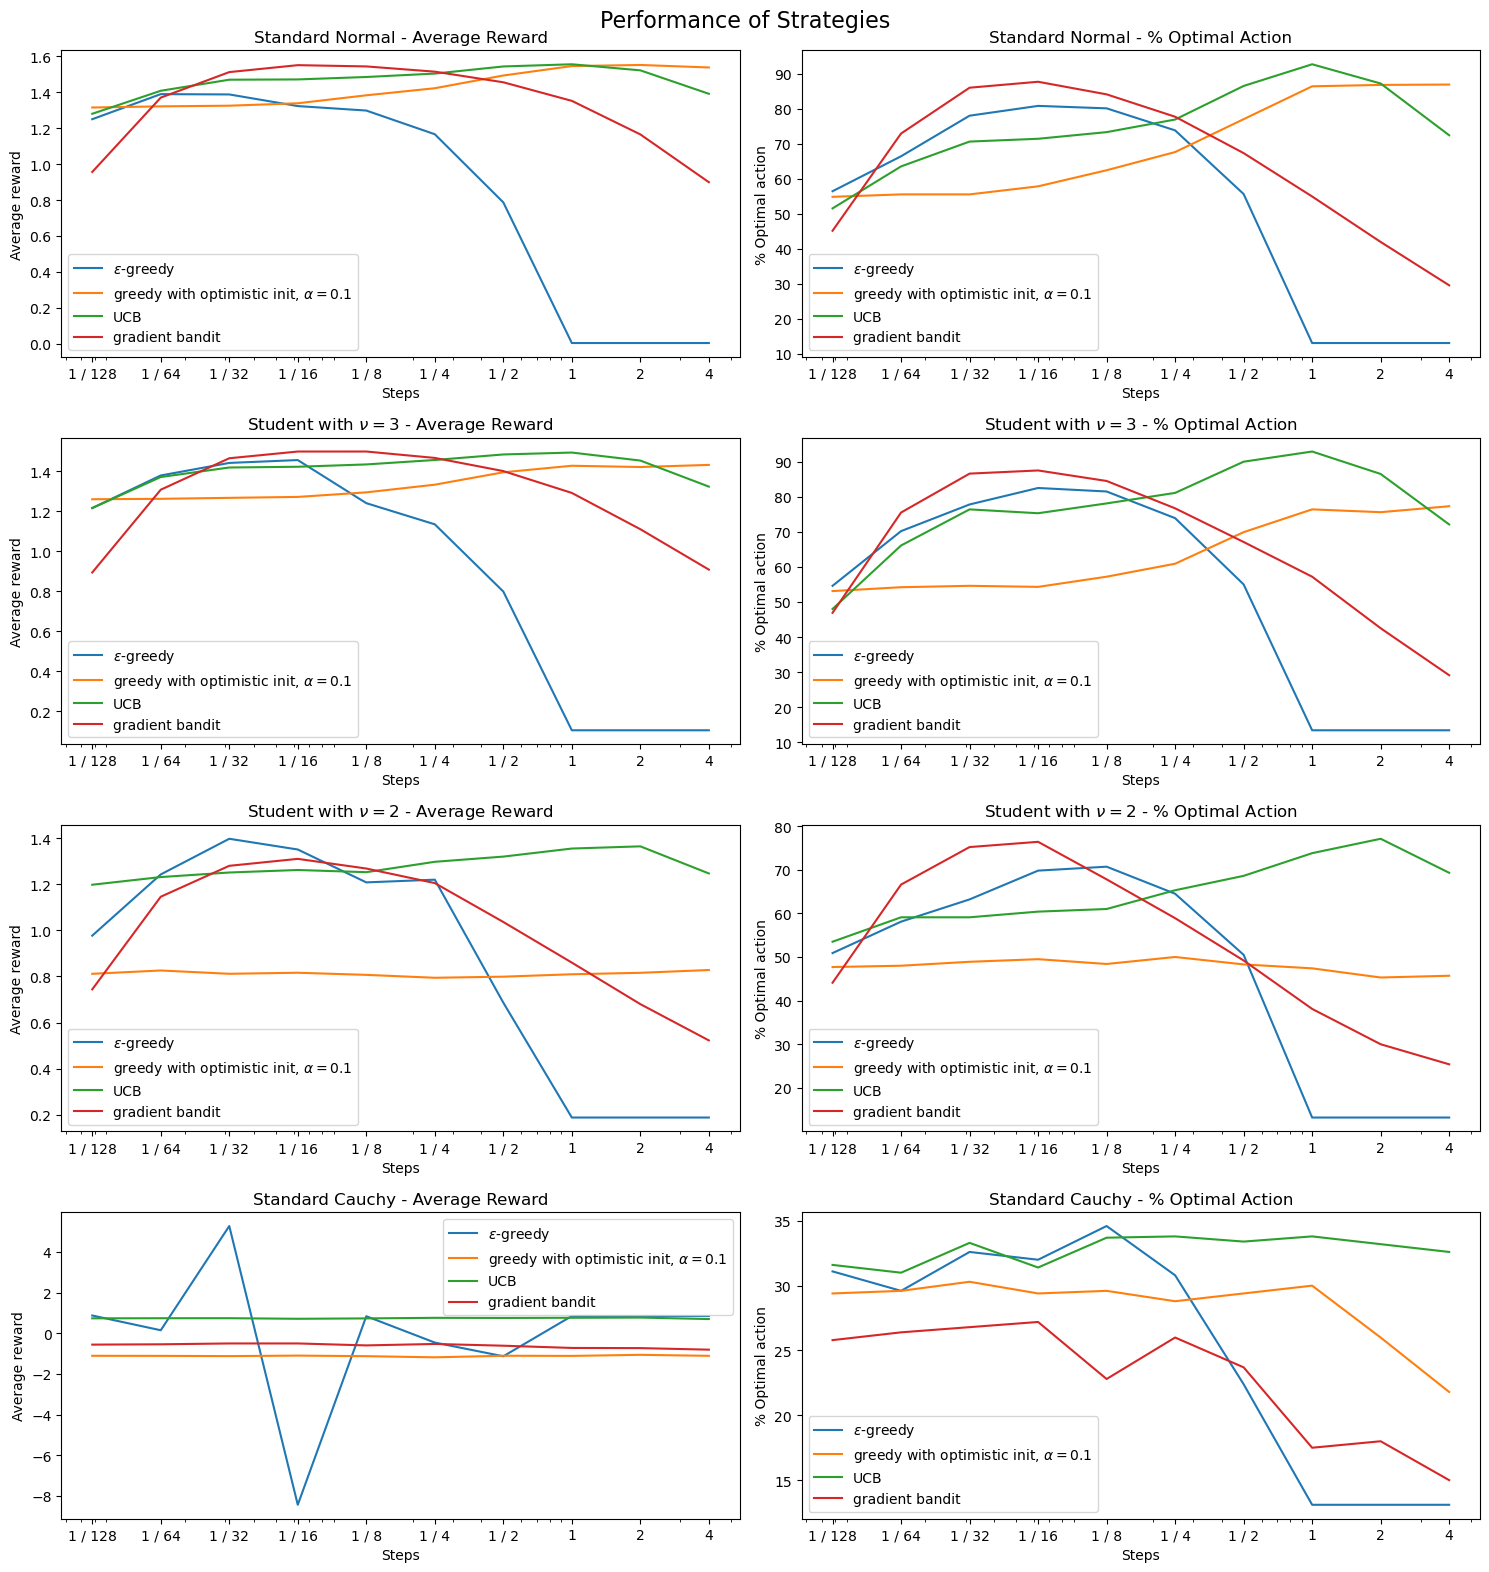
\includegraphics[width=1.1\linewidth]{overall.png}
    \caption{\label{fig:overall}Сравнение всех стратегий при варьировании гиперпараметров}
\end{figure}

Наконец, проанализируем графики со сравнениями всех стратегий. Для $t_{\infty}$ средняя награда достигает наибольшего значения для оптимистичной инициализации, gradient bandits и UCB, а процент оптимальных действий -- для UCB. Для $t_3$ ситуация такая же, за исключением того, что средняя награда для $\epsilon$-greedy достигает примерно таких же значений, что и для других стратегий. Для $t_2$ средняя награда и процент оптимальных действий для постоянного step-size значительно падают относительно других стратегий, что можно объяснить приданием одинакового значения выбросам выборки для любого шага. Средняя награда лучшая для $\epsilon$-greedy и UCB, процент оптимальных действий лучший для UCB и gradient bandits. Как я уже говорил, график средней награды для распределения Коши не имеет смысла, для процента оптимальных действий лучшие значения достигаются для $\epsilon$-greedy и UCB, при этом значения метрики для gradient bandits значительно падают относительно других стратегий и даже хуже, чем для стратегии с постоянным step-size. Так происходит, поскольку baseline есть среднее по всем предыдущим шагам, что не сходится ни к какому значению при любом распределении выбора действий.

В целом UCB на всех распределениях показывает лучший или один из лучших результатов, что можно объяснить тем, что эта стратегия дает любому рычагу воможность быть выбранным, при этом эта вероятность быть выбранным уменьшается с увеличением числа шагов и при этом в меньшей степени привязана к матожиданию, как, например, gradient bandits. Так как так же дается ненулевая вероятность быть выбранным каждому рычагу, $\epsilon$-greedy и gradient bandits тоже дают хорошие результаты на $t_2, t_3, t_{\infty}$.

\section{Выводы}

Проделанные эксперименты позволяют судить о том, что Gradient bandits, $\epsilon$-greedy и UCB -- стратегии показывают высокую эффективность на степенных распределениях. Так как UCB -- единственная из стратегий, показывающая высокую эффективность на всех метриках и всех распределений, то эта стратегия -- лучший из кандидатов для применения в оптимизации портфолио в модели прироста стоимости акций как многоруких бандитов.

\bibliographystyle{alpha}
\bibliography{RL.bib}

\end{document}